%My header and style options
\documentclass[a4paper, twocolumn, titlepage]{article}
\usepackage[slovene]{babel}
\usepackage[utf8]{inputenc}
\usepackage[T1]{fontenc}

%\usepackage{vicent}
%\usepackage[0T1]{fontenc}

%custom colour package
\usepackage[usenames, dvipsnames]{xcolor}

%graphics, captions etc.
\usepackage[pdftex]{graphicx}
\usepackage{amssymb, float, amsmath, fullpage, stackrel}

%to get the colourful hyperlinks ... not just square boxes around them ...
\usepackage{hyperref}
\hypersetup{
	colorlinks=true,
	linkcolor=black!60!red,
	citecolor=black!60!green,
	urlcolor=black!60!cyan,
	filecolor=black!60!magenta
}

%set up custom captions
\usepackage{caption}
\captionsetup{
	font=small,
	margin=10pt,
	labelfont=it,
%	labelsep=endash,
	format=hang,
	width=0.7\textwidth
}

%bibliography
%\usepackage[round]{natbib}

%LOOKS WAY BETTER WITHOUT THESE ... :P
%costum matter fonts and section fonts
%\usepackage{mathpazo}
%\usepackage{sectsty}
%\allsectionsfont{\LARGE\sffamily\bfseries}

\newcommand{\parc}[2]{
	\ensuremath{\frac{\partial#1}{\partial#2}}
}

\newcommand{\vac}[1][\phi]{
	\ensuremath{\langle#1\rangle}
}

%\renewcommand{\to}{
%	\ensuremath{\longrightarrow}
%}

% New definition of square root:
% it renames \sqrt as \oldsqrt
\let\oldsqrt\sqrt
% it defines the new \sqrt in terms of the old one
\def\sqrt{\mathpalette\DHLhksqrt}
\def\DHLhksqrt#1#2{%
\setbox0=\hbox{$#1\oldsqrt{#2\,}$}\dimen0=\ht0
\advance\dimen0-0.2\ht0
\setbox2=\hbox{\vrule height\ht0 depth -\dimen0}%
{\box0\lower0.4pt\box2}}

\newenvironment{myfig}[2][10cm]
{
	\vspace{-20pt}
	\begin{figure}[H]
		\begin{center}
			\includegraphics[keepaspectratio=1, width=#1]{#2}
		\end{center}
		\vspace{-24pt}
}
{
	\end{figure}
	\vspace{-6pt}
}

\renewenvironment{abstract}[1][1.0]
{
	\begin{center}\large
		{\bf Povzetek}\\[12pt]
		\begin{minipage}{#1\textwidth}
}
{
		\end{minipage}
	\end{center}
}

\newcommand{\rot}{
	\ensuremath{\vec{\nabla}\times}
}

\renewcommand{\div}{
	\ensuremath{\vec{\nabla}\cdot}
}

\newcommand{\ve}{
	\ensuremath{\vec{E}}
}

\newcommand{\vb}{
	\ensuremath{\vec{B}}
}

\newcommand{\w}{
	\ensuremath{\omega}
}

\renewcommand{\d}{
	\ensuremath{\mathrm{d}}
}

\begin{document}

%titlepage
\begin{titlepage}
	\begin{figure}[H]
		\centering
		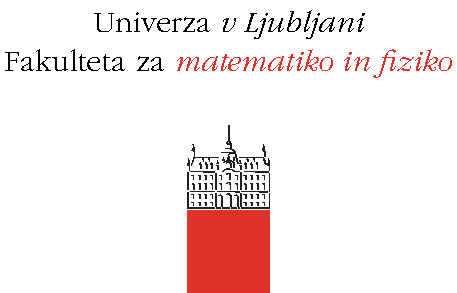
\includegraphics[width = 7cm, keepaspectratio=1]{pics/logo-slo.pdf}\\[12pt]
		\large{\sc Oddelek za fiziko}\\[4cm]
	\end{figure}
	\begin{center}
		\Large{Seminar -- 2. letnik 2. bolonjske stopnje}\\[0.5cm]
		\huge\textbf{Masivna elektrodinamika}\\[1.0cm]

		\vspace{0.0cm}

		\begin{minipage}{0.4\textwidth}\small
			\begin{flushleft}
				\large{\sc Avtor:}\\[0.2cm]
				\large{Jože Zobec}
			\end{flushleft}
		\end{minipage}
		\begin{minipage}{0.4\textwidth}\small
			\begin{flushright}
				\large{\sc Mentor:}\\[0.2cm]
				\large{Prof. Dr. Borut Bajc}
			\end{flushright}
		\end{minipage}
	\end{center}

	\vspace{4.5cm}

	\begin{abstract}
		Kot je verjetno potrebno venomer, so ob zori teorije o elektromagnetnem polju znanstveniki novosti
		sprejemali z zdravo mero dvoma. Tako so dlakocepili ob podrobnostih, ki so poznejše fizike privedle
		do možnosti neničelne mase fotona, katere eksperimentalno zaenkrat še ne moremo zanemariti. V tem
		seminarju bom na kratko opisal različne mehanizme, po katerih lahko foton dobi maso in naredil
		zgodovinski pregled meritev le-te.
	\end{abstract}
	
	\vfill

	\centering{\normalsize Ljubljana, \today}
\end{titlepage}

%table of contents, obviously ...
%\tableofcontents

\pagebreak

\section{Uvod}

Newtonova teorija gravitacije je s svojo učinkovitostjo ter preprostostjo narave presunila mnoge tedanje mislece in
služila za navdih novincem, ki so se tedaj ravno pričeli ukvarjati z elektrodinamiko. Predpostavka je bila, da
električna sila med naboji prav tako pada z $r^{-2}$, tako kot gravitacijska. Nekateri so temu oporekali in so
poskušali z $r^{-2 + \alpha}$, malenkost, ki je povezana prav z maso fotona.~\cite{nieto2}

Fiziki francoske šole so se o tem nekako največ spraševali. Med njimi prednjači Proca, ki je prvi zapisal ekvivalent
Maxwellovih enačb za masivne fotone~\cite{nieto1,over}. Za njim so se s tem ukvarjali Stueckelberg~\cite{over,nieto1},
de Broglie~\cite{nieto1,over}, in med drugimi tudi Schroedinger~\cite{nieto1}.

S pojavom kvantne elektrodinamike so poskušali slednjo uporabiti za masivne fotone, pri čemer so naleteli na
različne nevšečnosti, zaradi česar so pričeli z razvojem novih teoretičnih mehanizmov, s katerimi bi foton dobil maso
in hkrati ohranil lepe lastnosti brezmasne elektrodinamike.

Masivna elektrodinamika je tudi dandanes zanimiva, ker je eksperimentalno še ne moremo ovreči in nima daljnosežnih
posledic, kot jih imajo neabelove grupe ter gravitacija, zaradi česar jo lahko razumemo kot neke vrste uvod ali
predpripravo v fiziko masivnih vektorskih bozonov.

\section{Začetki elektrodinamike}

Maxwellove enačbe so nas dosegle konec devetnajstega stoletja, nekaj desetletij za tem, jih je Proca prepisal v obliko,
ki zado\v s\v ca neni\v celni fotonski masi. Ena\v cbe se potem glasijo

\begin{align}
	\div\ve &= \rho/\varepsilon_0 - m^2\varphi, \label{proca1} \\
	\div\vb &= 0, \label{proca2} \\
	\rot\ve &= -\parc{\vb}{t}, \label{proca3} \\
	\rot\vb &= \mu_0\vec{\jmath} + \frac{1}{c_0^2}\parc{\ve}{t} - m^2\vec{A}, \label{proca4}
\end{align}

kjer je $c_0 = 1/\sqrt{\varepsilon_0\mu_0}$ \v se vedno dobro definirana in nespremenjena. Odlej bom vse pisal v enotah
$\hbar = c_0 = \varepsilon_0 = 1$, saj so prikladnejše. Tu velja $E = \w$ in $\vec{p} = k_\mu$. Kot vidimo, so ena\v cbe Proca
v Lorentzovo kovariantni obliki nespremenjene za dualni napetostni tenzor elektromagnetnega polja, medtem ko dobi samo
divergenca napetostnega tenzorja masne popravke -- v Lorentzovo kovariantni obliki se torej prepišejo v

\begin{equation}
	\partial_\nu F^{\mu\nu} + m^2 A^\mu = -\jmath^\mu.
	\label{eqn:proca}
\end{equation}

\v Ce ena\v cbo \eqref{eqn:proca} diferenciramo, lahko od ondod dobimo pogoj za Lorentzovo umeritev, $\partial_\mu
A^\mu = 0$, ki nam reducira eno od \v stirih prostostnih stopenj $A^\mu$, od koder sledi, da gre za foton, s spinom $1$ in
maso $m$. Gostota Lagrangejeve funkcije\footnote{v nadaljevanju zaradi preprostosti raje kar Lagrangian}, $\mathcal{L}$,
se v tem primeru glasi

\begin{equation}
	\mathcal{L} = -\frac{1}{4}F_{\mu\nu}F^{\mu\nu} + \frac{1}{2}m^2A_\mu A^\mu.
	\label{eqn:proca-lagrangian}
\end{equation}

Vendar kot vidimo \v ze v en. \eqref{eqn:proca}, postanejo potenciali, torej $A_\mu = (\varphi, \vec{A})$ fizikalne
opazljivke v Lagrangianu~\eqref{eqn:proca-lagrangian}. Taka teorija nima umeritvene invariance, saj smo bili primorani
fiksirati v Lorentzovi skali.

\subsection{Posledice}

Kot sem namignil, ena\v cbe Proca s seboj prina\v sajo dolo\v cene nev\v se\v cnosti/
inovacije~\cite{nieto1,nieto2,stueckelberg}:

\begin{itemize}
	\item{kr\v senje umeritvene invariance,}
	\item{svetlobna disperzija}
	\item{pri visokih energijah postane teorija nerenormalizabilna,}
	\item{kr\v senje (lokalne) ohranitve naboja,}
	\item{dodatna longitudinalna komponenta elektromagnetnega sevanja,}
	\item{elektromagnetna interakcija ima kon\v cni doseg,}
\end{itemize}

kar nas lahko nekoliko preseneti -- da bo $\varphi$ dobil Yukawovo obliko gre pri\v cakovati, vendar kr\v senje ohranitve
naboja ni tako od muh. Pod kr\v sitvijo umeritvene invariance mislimo umeritveno invarianco prve vrste. Lagrangian zaradi
tega ni dober za kvantno relativistično kvantno mehaniko, saj tam dobimo divergence, ki jih ne moremo odpraviti z
renormalizacijo.

\subsubsection{Disperzijska relacija}

Svetlobna disperzija je najve\v cja razlika, ki jo je Proca povdarjal. Sam se ni menil, da bi ena\v cbe zapisal v
Lorentzovi kovariantni obliki in polja ni sku\v sal kvantizirati. Svetlobno disperzijo dobimo lahko na preprost
na\v cin~\cite{nieto1}:

\begin{equation}
	k_\mu k^\mu = \frac{\w^2}{c_0^2} - k^2 = m^2,
	\label{eqn:disper}
\end{equation}

kjer je $m$ masa fotona. \v Ce sedaj ena\v cbo~\eqref{eqn:disper} diferenciramo, lahko poka\v zemo da $\w \neq kc$, pri
\v cemer je 

$c = c_g = \mathrm{d}\w/\mathrm{d}k \neq c_0$ ($c = c_g$ je grupna hitrost takega vala). Po prej\v snjih ena\v cb sledi

\begin{equation}
	c = \sqrt{1 -\frac{m^2}{\w^2}} = \frac{|\vec{k}|}{\sqrt{|\vec{k}|^2 + m^2}},
	\label{disper2}
\end{equation}

od koder pa je o\v citno, da je $c = c (\w) \neq c_0$, ampak dobimo zaradi mase fotona majhne popravke. Prve meritve,
opravljene z namenom merjenja fotonske mase so bile
tako opravljene z merjenjem disperzije. Odslej bomo vse pisali v prej omenjenih normiranih enotah, kjer

\subsubsection{Kon\v cen doseg}

Proca ni vedel, da bi bila elektrodinamika tako zaradi Yukawovega potenciala kon\v cna in da bi to nato privedlo do
lokalne kr\v stve ohranitve elektri\v cnega naboja. Njegovim naslednikom je po Yukawovi napovedi `mezona' postalo jasno,
da bi dobili prav to. Da $\varphi$ res ustreza Yukawovemu potencialu, lahko vidimo, če enačbo~\eqref{proca1} zapišemo
za točkast naboj $(\rho = e\delta^3(\vec{r}))$ za stacionaren primer (časovni odvodi so enaki nič) in $\vec{E}$ nadomestimo s
potenciali~\cite{nieto2},

\begin{equation}
	\big(\nabla^2 - m^2\big)\varphi = -e\delta^3(\vec{r}), \quad \Longrightarrow \quad \varphi \propto
	\text{e}^{-\mu r}/r,
	\label{naboj}
\end{equation}

kar lahko enostavno rešimo\footnote{Hitro lahko opazimo, da je problem radialno simetričen $\Rightarrow \varphi =
\varphi(r)$. Ko enačbo rešimo, dobimo za rešitev superpozicijo sfernih Besselovih $j_n(x)$ Neumannovih
$y_0(x)$ funkcij za $x = imr$.
Uporabimo robni pogoj $\varphi(r) \stackrel{r\to\infty}{\longrightarrow}0$ in ugotovimo, da je $C_1 = 0$. Tako dobimo res
Yukawa potencial. Problem lahko rešimo tudi z Greenovo funkcijo, kar je še lažje in bolj neposredno.}.
Tak potencial je karakteristi\v cen za interakcije kon\v cnega dosega, kot je na primer \v sibka interakcija.

\subsubsection{Kr\v senje ohranitve naboja}

Gaussov zakon za ohranitev naboja dr\v zi v primeru, ko imamo potencial oblike $\varphi \propto 1/r$. Fotonska masa to
lepo lastnost seveda takoj pokvari, saj se \v stevilo silnic, ki prebadajo zaklju\v ceno ploskev ne ohranja, ampak se
spreminja. \v Ce je ta ploskev sfera s površino $\partial V$ (ki zaobjema volumen $V$), lahko zapi\v semo pretok
elektri\v cnega polja kot

\begin{multline}
	\Phi_e = \oint_{\partial V} \ve \cdot \d \vec{S} = \int_V \big(\div \ve\big)\ r^2\d r\ \d\Omega =\\=
		 m^2 \int_V \left(\frac{\text{e}^{-\mu r}}{r}\right)r^2 \d r = f(r) \neq e,
	\label{pretok}
\end{multline}

kjer smo se poslužili identitet iz en.~\eqref{naboj}.

\v Ceprav nekateri vir~\cite{nieto2} povdarja možnost kršitve lokalne ohranitve naboja v smislu $\partial_\mu\jmath^\mu 
\neq 0$, temu seveda ni tako, kar lahko pokažemo s pomočjo tega, da en.~\eqref{eqn:proca} odvajamo z operatorjem
$\partial_mu$,
kar nam vrne $\partial_\mu\jmath^\mu = 0$. To lahko demonstriramo tudi z izračunom divergence en.~\eqref{proca4},

\begin{align}
	\div(\rot\vb) &= 0 \notag \\
	&= \div\vec{\jmath} - m^2\div\vec{A} + \frac{\partial}{\partial t}\big(\rho - m^2\varphi\big) \notag \\
	&= \frac{\partial\rho}{\partial t} + \div\vec{\jmath} -m^2\Big(\underbrace{\frac{\partial\varphi}{\partial t} +
		\div\vec{A}}_{= \partial_\mu A^\mu = 0}\Big) \notag \\
	&= \partial_\mu\jmath^\mu = 0.
\end{align}

Sama gostota naboja se torej ohranja, vendar moramo za pravilno ohranitev upoštevati en.~\eqref{proca1}, in ne Maxwellove,
kar je jasno, saj lahko znova demonstriramo ohranitev, če integriramo po gostoto naboja $\rho(r)$, ki je porazdeljen 
po volumnu $V$:

\begin{align}
	e &= \int_V \d^3\vec{r}\rho(r) = \int_V \d^3\vec{r}(\div\ve + m^2\varphi) \notag \\
	&=\int_V\d^3\vec{r}\underbrace{(m^2 - \nabla^2)\varphi}_{e\delta^3(\vec{r})} = e,
\end{align}

kjer smo uporabili enačbo~\eqref{naboj}.
torej nam enačbe Proca res v primeru masivne elektrodinamike ohranjajo naboj. Kar je bilo verjetno mišljeno, je to da 
Maxwellove enačbe ne ohranjajo naboja, če imajo fotoni maso, kar pa pomeni natanko to, kar pravi en.~\eqref{pretok}.

\subsubsection{Longitudinalna polarizacija fotonov}

Brezmasna svetloba ima spin 1 in je vedno transverzalno polarizirana. To pomeni, da sta dovoljeni le projekciji $S = \pm 1$.

Projekcija $S = 0$ predstavlja longitudinalno polarizacijo. Zakaj ne more biti realizirana? Če je dovoljena, pomeni da se
lahko
gibljemo s tako hitrostjo, da bo val glede na nas miroval. V takem koordinatnem sistemu, bi izmerili $\vec{k} \equiv 0$.
V brezmasnem primeru tega ne moremo storiti, saj $c \equiv \w/|\vec{k}|$, kar nam očitno divergira za majhne $|\vec{k}|$.

V primeru za masivne fotone velja en.~\eqref{disper2}, ki nam dovoljuje takšno delovanje. Pove nam, da moramo svojo hitrost
izenačiti s hitrostjo fotona, kar je v soglasju s prejšnjim odstavkom. Longitudinalni fotoni imajo veliko
večjo penetracijsko moč, kot navadni žarki $\gamma$ (težje se obsorbirajo), verjetnost za izsevanje pa je sorazmerna z
maso fotona. Formalizem za njih je sicer enak, vendar niso bili opaženi, zaradi česar jih v nadaljnem ne bom omenjal.

\section{Stueckelbergov mehanizem}

V dvajsetih letih prej\v snjega stoletja je Stueckelberg demonstriral kako lahko splo\v snemu kompleksnemu vektorskemu
polju, ki ima simetrijo U(1), dodamo maso, ne da bi pri tem zlomili umeritveno invarianco in hkrati ohranili
renormalizabilnost teorije. Njegove ideje so ostale v ozadju, a so pozneje slu\v zile za navdih Higgsovemu mehanizmu.
Njegovo idejo so seveda uporabili tudi za realno vektorsko polje, $A_\mu$, se pravi foton.

Stueckelberg si je mislil, da je tisto kar je najpomembnej\v se v teoriji to, da je umeritveno invariantna. Pri tem imamo
lahko ve\v c razli\v cnih umeritev: umeritve skale~\cite{stueckelberg,nieto2}, umeritve faze~\cite{nieto2} \ldots Njegova
teorija ohranja oboje. Trik za foton
uporabimo takole: ker vemo, da mora imeti masivno vektorsko polje s spinom 1 prisotne natanko 3 prostostne
stopnje\footnote{spine, polarizacije}, se mu je zdelo primernej\v se pri\v ceti z $A_\mu$, kot pa z $F_{\mu\nu}$.
Rekel je: za masivni foton $A_\mu$ mora veljati Klein-Gordonova enačba:

\begin{equation}
	(\Box + m^2)A_\mu (x) = 0,
\end{equation}

$A_\mu$ ima
4 prostostne stopnje. Proca se je ene stopnje znebil s pomo\v cjo Lorentzove umeritve, Stueckelberg pa tega pogoja tukaj ni
dobil, zato je moral vpeljati novo skalarno polje $B$, ki je povezano z $A_\mu$ prek iste\footnote{To je bilo res za
enačbe, kot jih je zapisal on, po Feynamu in t'Hofftu, pa se v Lagrangiane dodaja še člene, ki nam dopuščajo umeritev
skale -- $\xi$.} Klein-Gordonove enačbe,

\begin{equation}
	(\Box + \xi m^2)B (x) = 0, \quad \xi \in \mathbb{R}.
	\label{kg}
\end{equation}

Tako imamo naenkrat 5 prostostnih stopenj. Izka\v ze se, da lahko na tem mestu postuliramo relacijo

\begin{equation}
	\big[\partial_\mu A^\mu(x) + \xi mB(x)\big]^{(-)}|\phi\rangle = 0,
	\label{qed:lorentz}
\end{equation}

kjer je $|\phi\rangle$ katerokoli fizikalno stanje, operatorji pa imajo gornji indeks `$-$', ki ponazarja da gre le za
anihilacijske operatorje. Izraz~\eqref{qed:lorentz} je posplošitev izraza iz kvantne elektrodinamike, le da je tam $m = 0$,
kar naredi teorijo privlačno. S tem se znebimo ene od prostostnih stopenj, ko pa polje kvantiziramo opazimo, da imamo
umeritveno svobodo, ki nam skupaj zreducira \v stevilo prostostnih stopenj na 3. Dovoljena umeritev faze je te vrste:

\begin{align}
	A_\mu (x) &\to A_\mu (x) + \partial_\mu \Lambda (x), \notag \\
	B (x) &\to B (x) + m\Lambda(x), 
\end{align}

kjer mora $\Lambda (x)$ prav tako rešiti en.~\eqref{kg}, se pravi 

\begin{equation}
	(\Box + \xi m^2)\Lambda(x) = 0.
	\label{umeritev}
\end{equation}

Če bi hoteli torej popraviti Lagrangian Proca~\eqref{eqn:proca-lagrangian}, bi tem transformacijam ustrezala substitucija

\begin{equation}
	A_\mu (x) \to A_\mu (x) - \frac{1}{m}\partial_\mu B(x),
\end{equation}

ki nam vrne Lagrangian

\begin{equation}
	\mathcal{L} = -\frac{1}{4}F_{\mu\nu}F^{\mu\nu} + \frac{1}{2}m^2\Big(A_\mu - \frac{1}{m}\partial_\mu B\Big)^2.
\end{equation}

Vendar pa je ta Lagrangian umeritveno invarianten (členi s $\xi$ v enačbah~\eqref{kg},~\eqref{qed:lorentz}
in~\eqref{umeritev}, zaradi česar moramo dodati še člene, ki nam fiksirajo skalo (ang. gauge fixing). Končni Lagrangian,
kateremu lahko potem spreminjamo tako fazo, kot skalo, se potem zapiše kot

\begin{multline}
	\mathcal{L} = -\frac{1}{4}F_{\mu\nu}F^{\mu\nu} + \frac{1}{2}m^2\Big(A_\mu - \frac{1}{m}\partial_\mu B\Big)^2 -\\-
		\frac{1}{2\xi}\big(\partial_\mu A^\mu + \xi mB\big)^2,
\end{multline}

ki je spet zvezna posplošitev Lagrangiana za brezmasne fotone.

Poleg tega, da ohranimo svobodo umeritve ima Stueckelbergov trik \v se eno lepo lastnost: $F_{\mu\nu} F^{\mu\nu}$ je enak,
saj se prispevki skalarnega polja ravno izni\v cijo. Novo skalarno polje $B(x)$ interpretiramo kot longitudinalno polarizacijo
fotona.

\section{Higgsov mehanizem}

Higgsov mehanizem prav tako lahko reši Lagranian Proca~\eqref{eqn:proca-lagrangian} in prav tako doda novo skalarno polje,
vendar je tam ideja druga\v cna: vse skupaj je mogo\v ce prek spontanega zloma simetrije.

Higgsovega mehanizma ne gre me\v sati s Higgsovim delcem, katerega kandidata so v leto\v snjem poletju odkrili v CERN-u.
Foton sam pripada grupi U(1) in za maso ne potrebuje takega mehanizma -- maso dobi neodvisno.

Prva taka razlika od elektro\v sibkega Higgsa je ta, da je elektromagnetni Higgs tu elektri\v cno nabit delec. Njegov
naboj je sorazmeren z maso fotona.

Zaradi sorodnosti s superprevodniki bi v tem primeru tudi pomenilo, da je masa fotonov lahko temperaturno odvisna in pri
neki kriti\v cni temperaturi postane enaka ni\v c (superprevodna faza fotonov).

Zaenkrat eksperimentalno nič ne kaže, da bi Higgsov mehanizem bil prava pot, vendar pa kot je bilo demonstrirano
v~\cite{higgs}, so dosedanje kozmološke meritve nezadostne.

Lagrange-ian~\eqref{eqn:proca-lagrangian} torej ni invarianten na transformacije $A_\mu (x) \to A_\mu (x) +
\partial_\mu\Lambda(x)$. Namesto da bi maso dodali v Lagrangeian direktno, s členom $\frac{1}{2}m^2 A_\mu A^\mu$, bomo
raje vpeljali novo skalarno polje $\phi$ z elektromagnetno interakcijo (nabojem $q$). Če torej vpeljemo kovariantni
odvod $D_\mu = \partial_\mu - iqA_\mu$ in $V(\phi) = -\mu^2 \phi^\dagger\phi + \lambda(\phi^\dagger\phi)^2$ dobimo
Lagrangian

\begin{equation}
	\mathcal{L} = -\frac{1}{4}F^{\mu\nu}F_{\mu\nu} + (D_\mu\phi)^\dagger(D^\mu\phi) - V(\phi),
	\label{eqn:higgs-lagrangian1}
\end{equation}

ki je invarianten na umeritvene transformacije

\begin{align}
	A_\mu(x) \to& A_\mu(x) + \partial_\mu \Lambda(x), \notag \\
	\phi(x) \to& \text{e}^{iq\Lambda(x)}\phi(x).
\end{align}

Če je ima $\mu^2 > 0$ v $V(\phi)$ je minimum energije pri $\langle \phi \rangle_\pm = \pm \sqrt{\mu^2/2\lambda} \equiv \pm
v/\sqrt{2}$. Tako smo dobili pričakovano vrednost vakuuma, $v$. S pomočjo te vrednosti lahko parametriziramo $\phi$ kot

\begin{equation}
	\phi(x) = \frac{v + h(x)}{\sqrt{2}}\mathrm{e}^{i\chi/v}.
\end{equation}

Ta izraz vstavimo v en.~\eqref{eqn:higgs-lagrangian1} in tako dobimo

\begin{align}
	\mathcal{L} =& -\frac{1}{4}F^{\mu\nu}F_{\mu\nu} + \frac{q^2v^2}{2}A^\mu A_\mu + \notag \\
	&+ \frac{1}{2}(\partial_\mu h)(\partial^\mu h) - \mu^2 h^2 + \notag \\
	&+ \frac{1}{2}(\partial_\mu\chi)(\partial^\mu\chi) - qvA_\mu\partial^\mu\chi \notag \\
	&+ (\text{interakcije $\chi - h$, $h - A_\mu$ in $h - h$}).
	\label{eqn:higgs-lagrangian}
\end{align}

Kot vidimo, dobi v en.~\eqref{eqn:higgs-lagrangian} foton maso $q^2\mu^2 = m^2$, vendar se moramo znebiti še člena $\chi$,
ker nam mešajo $A_\mu$ in $\partial_\mu \chi$. To storimo s tako izbiro umeritve

\begin{equation}
	A_\mu \to A_\mu - \frac{1}{qv}\partial_\mu\chi,
\end{equation}

ki ji pravimo unitarna umeritev. Ta $\chi$ je bil brezmasni Nambu-Goldstonov bozon, ki je bil posledica spontanega zloma
simetrije. Ko se ga znebimo z umeritvijo, pravimo da je bil absorbiran v fotonsko maso in je "`would-be"' Goldstonov bozon.

Tudi v tem primeru pravimo, da novo realno skalarno polje $\chi$ da maso fotonu $A_\mu$ in ga prav tako interpretiramo kot
longitudinalno polarizacijo.

\section{Izvleček teorije}

Lagrangian Proca, en.~\eqref{eqn:proca-lagrangian}, je torej slab iz teorijskega vidika, saj nam ne omogoča kvantne
elektrodinamike -- pri visokih energijah ima divergence, ki se jih ne moremo znebiti s standardnim renormalizacijskim
postopkom. Ima tudi druge nevšečnosti, ki pa so bolj matematične narave.

Ko želimo te nevšečnosti popraviti so nam na voljo mnogi triki, najbolj se uporabljata Stueckelbergov in pa Higgsov mehanizem.
Oba imata sorodno to, da dodamo neko novo realno skalarno polje $\psi(x)$, s katerim transformiramo
Lagrangian~\eqref{eqn:proca-lagrangian}

\begin{equation}
	A_\mu(x) \to A_\mu(x) - \frac{1}{m}\psi(x),
\end{equation}

ki ga interpretiramo kot longitudinalno polarizacijo fotona. Vendar je med njima opazljiva fizikalna razlika -- Stueckelberg
doda zgolj novo polarizacijo, Higgs pa poleg tega doda še novo fizikalno polje, oz. nov Higgsov delec. Higgsov mehanizem
dopušča temperaturno spreminjanje mase fotona, kar je Stueckelbergovemu Lagrangianu tuje.

Obe teoriji zvezno posplošita brezmasni primer, kar pomeni, da je lahko maso fotona zvezno limitiramo proti 0 in pri obeh
primerih dobimo nazaj kvantno elektrodinamiko in Maxwellove enačbe.

\section{Meritve}

Nikoli ne moremo eksaktno izmeriti, da je masa fotona 0. Lahko določujemo samo zgornjo mejo. Vendar pa vseeno obstaja neka
meja, do kod se jo splača meriti -- dobimo jo s Heisenbergovim principom
neenakosti~\cite{over}:

\begin{equation}
	\delta t \cdot \frac{\delta E}{\hbar} = \delta t \cdot \frac{mc_0^2}{\hbar} = \delta t \cdot \mu c_0 \sim 1,
\end{equation}

kjer za $\delta t$ vstavimo starost vesolja ($10^{17}$ sekund) in dobimo spodnjo mejo za maso fotona \hbox{$m \sim
10^{-69}$ kg}.
\v Ce je masa fotona manj\v sa od tega, pomeni da jo lahko pripi\v semo kvantnim fluktuacijam, katere pa \v ze znamo
pojasniti in bi bile meritve odve\v c.

Meritve lahko združimo nekako v tri razrede:
\begin{itemize}
	\item{Laboratorijske -- opravljene so v skrbno nadzorovanem okolju na Zemlji.}
	\item{Meritve znotraj na\v sega oson\v cja -- opravljene so s pomočjo satelitov.}
	\item{Kozmološke -- s teleskopi opazujemo razna nebesna telesa, ki so zelo oddaljena.}
\end{itemize}

Laboratorijske lahko nato razdelimo še na `kvantne' in `klasične', kjer pod klasične mislimo spremembe glede na Maxwellovo
elektrodinamiko.

\subsection{Laboratorijske meritve}

Vse skupaj se je pričelo s preverjanjem odvisnosti $F \propto r^{-2}$. Ker so fiziki tedaj pluli v neznane vode, so dopuščali
popravek temu, tj. $r^{-2 + \alpha}$. V primeru fotonske mase se izkaže, da je $\alpha = \alpha (r)$, ker je potencial
masivnega fotona oblike $\varphi \sim \text{e}^{-\mu r}/r$. Odklone od zakona $r^{-2}$ so merili predvsem na dva načina:
\textbf{(a)} direktno z meritvijo pojemanja sile z razdaljo (Coulomb, Robinson), \textbf{(b)} z merjenjem odsotnosti sil
zunanjih lupin znotraj sferičnega objekta\footnote{Kot je Newton demonstriral za svojo teorijo gravitacije, ima sila obliko
$F \sim r^{-2}$, kar prinaša s seboj lepe lastnosti: če smo namreč na neki globini $h$ pod Zemljo, na nas deluje le sila
Zemlje z radijem $R - h$, se pravi, da nam zunanje lupine z debelino $h$ ni treba upoštevati, ker je njen prispevek natanko
0. Ko so to prevedli na meritve električnih sil, v veliko nabito kroglo zaprli manjšo in opazovali interakcije med njima --
po navadi pretečen električni naboj.} in merjenjem oblike električnega potenciala (Cavendish, Maxwell \ldots). Te meritve so
očitno laboratorijske. V zadnjih dveh, treh desetletjih so pričeli meriti tudi kvantne posledice.

\subsubsection{Klasične meritve}

Meritve odklona tipa $F \sim r^{-2 - \alpha}$ lahko povežemo z meritvami fotonske mase, ker lahko izpeljemo
enakost~\cite{over}

\begin{equation}
	\frac{\varphi(r) - \varphi(a)}{\varphi(a)} \approx \alpha(r) \approx -\frac{1}{6}\mu^2(a^2 - r^2),
\end{equation}

kjer je $\mu$ recipročna Comptonova dolžina fotona, ki je z maso povezana kot $m = \mu\hbar/c_0$. Od tod lahko s poznavanjem
dimenzij problema dobimo podatek o masi takega fotona.

Franklin (1755) je naredil prvi eksperiment, kjer je na nitki obesil majhno plutovinasto kroglico in dal, da je visela v nabit
kovinski lonček~\cite{over}. Ker ni bilo interakcije med njima, je Priestley (1767) sklepal, da sila pada s kvadratom
razdalje, tako kot Newtonova gravitacijska sila, ker bi se v tem primeru prispevki sil izničili. Eksperiment je bil zgolj
kvalitativen in je služil zgolj kot motivacija naslednikom.

Prvo kvantitativno obravnavo je naredil Škotski fiziolog Robison (1769). Meril je odbojno silo med dvemi nabitimi palicami,
ki jo je uravnovesil z njuno privlačno gravitacijsko silo -- maso palic je namreč poznal. Izmeril je odklon $\alpha = 0,06$
in tudi ugibal, da bi morala biti ta številka negativna za privlačno električno silo, zaradi česar je sklepal da je $r^{-2}$
res pravi zakon. Rezultate je objavil šele leta 1801, 13 let za Coulombom, dasiravno je meritev opravil pred njim.

Coulombov poskus (1788) je bil bolj sofisticiran, meril je odbojno, kot tudi privlačno silo električno nabitih krogel s
pomočjo torzijske tehtnice. Odmik zaradi sile, je torej prenesel na odmik kota, ki ga je meril z zrcalom, na katerega je
imel usmerjen svetlobni snop. Njegov rezultat je ustrezal $\alpha \leq 0,01$.

Vsi drugi klasični laboratorijski poskusi so bili sorodnega tipa, kot si ga je zamislil Cavendish. Njegov eksperiment
je bil zastavljen takole: imel je dve koncentrični krogli, zunanja je bila sestavljena iz dveh polobel, da se jo je lahko
razprlo. Znotraj sta bili povezani z elektrostatsko napravo~\cite{over}. Povezavo so nato nenadoma prekinili, zunanjo kroglo
previdno odprli in preverili, če je naboj notranje krogle res enak 0. Cavendish je dobil rezultat $\alpha \leq 0,02$, torej
slabše od Coulomba.

Isti poskus pozneje opravil tudi Maxwell in za rezultat dobil $\alpha \approx 5 \times 10^{-5}$.

Poskus so opravili nato z raznimi koncentričnimi telesi, ne le s kroglami, saj v primeru $r^{-2}$ Gaussov zakon velja za vse
oblike. Tako so isto stvar ponovili s kockami, ikozaedri in na izmeničnih napetostih s fazno vpeto zanko (Plimpton in
Lawton -- 1936, Cochran in Franken -- 1968,  Bartlett in Phillips -- 1969, Williams, Faller in Hill -- 1971).

V laboratorijih so skušali opraviti tudi poskuse svetlobne disperzije, vendar se bolj obnesejo pri velikih razdaljah in
zategadelj spadajo med astronomska opazovanja.

\subsubsection{Kvantni poskusi}

To so poskusi, katere je fizikom šele pred kratkim uspelo narediti in so privlačni zaradi tega, ker jih lahko izvajamo v
nadzorovanem okolju.

Meritve, ki so bile opravljene z zadovoljivo natančnostjo, so bile Aharonov-Bohm efekt in defekti giromagnetnega razmerja
elektrona. Pri giromagnetnem razmerju rezultat izgleda prigoljufan. Masa fotona, dobljena na ta način, je namreč zelo groba
ocena in ne namenska meritev fotonske mase. Ocenijo jo namreč tako, da vse odstopanje meritve od teoretične vrednosti, ki jo
napoveduje kvantna elektrodinamika za brezmasni foton, pripišejo fotonski masi. Napaka meritve je
$\Delta g \sim 10^{-14}$~\cite{over}. Vrednost, ki so jo dobili na ta način je $m \approx 10^{-54}$ g~\cite{over}.

Pri Aharonov-Bohm efektu gre za pravo in bolj sofisticirano meritev. Zaradi efektov kvantne mehanike se je izkazalo, da
lahko namreč merimo vpliv vektorskega potenciala magnetnega polja na fazo interferenčne dveh vzporednih elektronskih curkov,
ki med katerima je pravokotno na njuno tirnico postavljen solenoid. Ta efekt ima teoretično napoved za neničelno, kot tudi
ničelno maso fotona. Najnatančnejši rezultat so dobili Williams, Faller in Hill (1965), $m \lesssim 10^{-14}$ eV $\equiv
2\times 10^{-47}$ g~\cite{nieto2}, čeprav so dobili tudi že nižje vrednosti $m \sim 10^{-51}$ g~\cite{over},
$m \sim 10^{-51}$ g, $m \sim 10^{53}$ g in tudi $m \sim 10^{54}$ g (skalarni Aharonov-Bohm efekt~\cite{over}).

Take meritve postajajo končno primerljive z opazovanji iz vesolja in bodo morda prinesle merjenje fotonske mase nazaj na
Zemljo.

Kot zanimivost naj dodam tudi to, da so po navdihu Higgsovega mehanizma za foton naredili tako imenovani "`kriogenski"'
poskus tipa Cavendish. Teoretični princip za temperaturno odvisnost sta napisala Primack in Scher~\cite{nieto2},
opravili pa so ga Ryan, Acceta in Austin (1985) in dosegli $m \leq (1,5 \pm 1,38) \times 10^{-42}$ g, pri temperaturi
$1,36$ K~\cite{over}.

\subsection{Meritve v našem osončju}

Fiziki prejšnjega stoletja so videli, da je Maxwellova elektrodinamika zelo natančna v skoraj vseh pogledih. Možnosti za
nadgradnjo so videli bodisi pri zelo velikih razdaljah\footnote{zelo dolga valovna dolžina}, bodisi pri rešitveh po dolgem
času.

Schroedinger (1943)~\cite{nieto1} se je zato odločil, da bo meril obliko silnic zemeljskega magnetnega polja. Dipolni moment
Zemlje bi po Maxwellu imel obliko $1/r^3$, vendar pa mora zaradi Yukawovega potenciala padati hitreje. Defekt bi bil najbolje
viden na ekvatorju. Schroedinger je uporabil že obstoječe meritve iz leta 1922, ki jih je objavil gospod Schmidt leta 1924.
Leta 1955 sta se z Bassom odločila, da bosta rezultat pomnožila s faktorjem $2$ in dobila mejo $m \leq 10^{-47}$
g~\cite{nieto1}.

Schroedingerjevo meritev sta ponovila A. S. Goldhaber in M. M. Nieto (1968) in dobila oceno $m = 4 \times 10^{-48}$
g~\cite{nieto1, over}.

Iste poskuse so pozneje opravili za večja telesa, kot je tudi Schroedinger predlagal. Najboljši rezultat bi po njegovem
mnenju dal Jupiter, saj je največji med planeti. To je storil Davis (1975) s svojo ekipo, uporabili so rezultate sonde
Pioneer in dobili rezultat $m \lesssim 4\times10^{-16}$ eV $\equiv 7 \times 10^{-49}$ g~\cite{nieto2,over}.

S pomočjo disperzije optične svetlobe je de Broglie napovedoval mejo $m \leq 10^{-39}$ kg~\cite{nieto2}. Pozneje jo je
izmeril Kroll, ki pravi $m \lesssim 3 \times 10^{-13}$ eV $\equiv 4 \times 10^{-46}$ g~\cite{nieto2}.

Opravljene so bile še druge meritve, ki so predolge za ta seminar, kot na primer vplivi mase na sončev veter (Ryutov 2007,
$m \lesssim 10^{-18}$ eV $\equiv 2\times10^{-51}$ g).

\subsection{Kozmološke meritve}

Pod tem imenom je mišljeno na meritve, ki so galaktičnih razsežnosti, izven našega osončja. Meri se predvsem magnetno polje in
vektorski potencial iz galaktičnega jedra~\cite{over}, obliko svetlobnega snopa iz pulzarjev~\cite{nieto1} in oblike
meglic~\cite{nieto2}. V članku~\cite{higgs} je razloženo, da so ta opazovanja v primeru elektrodinamskega Higgsa nična in
ne merijo mase fotona.

Najzanimivejša metoda je metoda, ki jo je predlagal Lakes (1998) za merjenje magnetnega vektorskega potenciala. Magnetno
polje je daleč od galaktičnega jedra skoraj konstantno, prav tako tudi vektorski potencial, ki je zaradi mase fotona
opazljivka v Lagrange-ianu. Zaradi vrtenja Zemlje okrog svoje osi s frekvenco $\w$ in neničelnega ambientalnega vektorskega
potenciala, bi na Zemljo deloval navor

\begin{equation}
	\vec{M} \propto \vec{\w} \times m^2\vec{A}
\end{equation}

Smer $\vec{A}$ lahko sklepamo iz smeri vrtenja naše galaksije, dolžino pa je ocenil s z $|\vec{A}| \approx L|\vec{B}|$, kjer
je $L$ oddaljenost od galaksije. Ravno zaradi teh predpostavk ne moremo biti gotovi v rezultate meritve -- lahko da je
$\vec{A}$ veliko manjši od $LB$, prav tako ne vemo če je magnetno polje res homogeno. Kljub temu so po njegovem predlogu
naredili meritev in dobili $m \lesssim 7 \times 10^{-20}$ eV $\equiv 10^{-52}$ g~\cite{nieto2}. Ker seveda ne poznamo prave
vrednosti $\vec{A}$ je to zelo groba ocena. Če je $|\vec{A}|$ zelo majhna vrednost, ne bi opazili mase fotona, tudi če bi
bila zelo velika. Prav tako ne moremo reči, da je celoten prispevek $\vec{A}$ posledica vektorskega potenciala galaksije.

Higgsov mehanizem bi bil tudi tukaj -- v režimu, ki bi bil analogen superprevodniku tipa II, bi imel foton maso lahko v zelo
visokih energijah, temperaturah, torej v zgodnjem vesolju~\cite{nieto2}.

\section{Izvleček eksperimentov}

Particle Data Group~\cite{pdg}, ki vodi almanah za rezultate meritev in "`uradne izmerjene vrednosti ta hip"', o fotonu pove
sledeče:

\begin{itemize}
	\item{{\bf Najbolj gotova vrednost:} izmeril Ryutov, $m < 10^{-18}$ eV, z merjenjem hidromagnetnih pojavov Sončevih
		vetrov. Zatrjujejo, da z metodo merjenja zaobjel področje do radija Plutonove orbite. To je največje
		magnetno polje, kar nam je na voljo, zato je tudi ta meritev najbolj čislana.}
	\item{{\bf Doslej najnižja izmerjena vrednost:} izmeril Chibisov, $m < 3\times10^{-27}$ eV, z merjenjem galaktičnega
		magnetnega polja.}
	\item{{\bf Najbolj natančna meritev:} Davis, $m < 6\times10^{-16}$ eV, ki dodaja še stopnjo zaupanja $99,6\%$, z
		merjenjem Jupitrovega magnetnega polja.}
\end{itemize}

\section{Zaključek}

Verjetno še vedno kakih sto let proč, preden bo dosežena
Heisenbergova meja $m \sim 10^{-66}$ g. Trenutno se Higgsov sektor nekako prebuja in fiziki skušajo odstopanja od klasične
Maxwellove elektrodinamike parametrizirati s Higgsovim mehanizmom za nadaljne meritve. Opravljene so bile še mnoge druge
meritve, nekatere bolj eksotične od teh sploh v kozmoloških opazovanj, tudi teorija v ozadju je v mnogih bolj divja, sploh
pri Higgsovem mehanizmu~\cite{higgs}. 

%Zgodovinski pregled eksperimentov si lahko pogledate na sliki~\ref{pic}
%
%\begin{figure}[H]\centering
%	\includegraphics[keepaspectratio=1, width=\0.8\textwidth]{pics/slika.png}
%	\caption{Zgodovinski limitiranja fotonske mase proti 0.}
%	\label{pic}
%\end{figure}

\begin{thebibliography}{9}
	\bibitem{nieto2}
	A. S. Goldhaber and M. M. Nieto,
	"`Photon and Graviton Mass Limits"',
	arXiv:0809.1003v5 [hep-ph]
	(2010)

	\bibitem{nieto1}
	A. S. Goldhaber and M. M. Nieto,
	"`Terrestrial and Extraterrestrial Limits on The Photon Mass"',
	Rev. Mod. Phys. {\bf 43}, 277-296
	(1971)

	\bibitem{stueckelberg}
	H. Ruegg and M. Ruiz-Altaba,
	"`The Stueckelberg Field"'
	arXiv:hep-th/0304245v2
	(2003)

	\bibitem{over}
	G. Spavieri, J. Quintero, G.T. Gillies and M. Rodriguez,
	"`A survey of existing and proposed classical and quantum approaches to the photon mass"',
	Eur. Phys. J. D {\bf 61} 531-550
	(2011)

	\bibitem{higgs}
	E. Adelberger, G. Dvali and A. Gruzinov,
	"`Photon Mass Bound Destroyed by Vortices"',
	arXiv:hep-ph/0306245v2
	(2003)

	\bibitem{pdg}
	J. Beringer et al. (Particle Data Group),
	Phys. Rev. {\bf D86}, 010001,
	(2012)
	(URL:http://pdg.lbl.gov)
\end{thebibliography}

\end{document}

